
%(BEGIN_QUESTION)
% Copyright 2010, Tony R. Kuphaldt, released under the Creative Commons Attribution License (v 1.0)
% This means you may do almost anything with this work of mine, so long as you give me proper credit

Predict the effects of steam demand suddenly increasing in this boiler system (i.e. loads drawing more steam flow from the boiler than before).  Assume all loop components are properly configured, that the controller is well-tuned, and that a significant amount of time has passed since the steam demand changed.  Compare these conditions with what they were before the process change:

$$\includegraphics[width=15.5cm]{i02001x01.eps}$$

\begin{itemize}
\item{} Feedwater valve will: {\it open up} further, {\it close down} more, or {\it remain in the same position}
\vskip 10pt
\item{} Steam drum water level will: {\it increase} from what it was before, {\it decrease} from what it was before, or {\it remain the same} as before
\end{itemize}

\underbar{file i02001}
%(END_QUESTION)





%(BEGIN_ANSWER)

\begin{itemize}
\item{} Feedwater valve will: {\bf open up further}
\vskip 5pt
\item{} Steam drum water level will: {\bf remain the same as before}
\end{itemize}

%(END_ANSWER)





%(BEGIN_NOTES)

{\bf This question is intended for exams only and not worksheets!}.

%(END_NOTES)


